\documentclass{ctexart}
\usepackage{subfig,amsmath,amsthm,amssymb,bm,graphicx,hyperref,mathrsfs,algorithmic,algorithm,listings,xcolor,geometry} 
\definecolor{mygreen}{rgb}{0,0.6,0}
\definecolor{mygray}{rgb}{0.5,0.5,0.5}
\definecolor{mymauve}{rgb}{0.58,0,0.82}
\lstset{ %
	backgroundcolor=\color{white},      % choose the background color
	basicstyle=\footnotesize\ttfamily,  % size of fonts used for the code
	columns=fullflexible,
	tabsize=4,
	breaklines=true,               % automatic line breaking only at whitespace
	captionpos=b,                  % sets the caption-position to bottom
	commentstyle=\color{mygreen},  % comment style
	escapeinside={\%*}{*)},        % if you want to add LaTeX within your code
	keywordstyle=\color{blue},     % keyword style
	stringstyle=\color{mymauve}\ttfamily,  % string literal style
	frame=single,
	rulesepcolor=\color{red!20!green!20!blue!20},
	% identifierstyle=\color{red},
	language=Verilog,
}
\geometry{a4paper,left=2.5cm,right=2.5cm,top=2cm,bottom=2cm}
\title{OooooS小组选题和调研报告}
\author{罗浩民\;陈琳波\;赵于洋\;刘时\;李丁}
\date{\today}

\begin{document}
\maketitle

\section{前言}
随着计算机科学与计算机工艺的不断进步,计算机内的可用资源逐渐增多。与此同时,用户对计算机的要求也逐渐多样化,从以前的重复计算,到足不出户访问世界,再到人机交互等等。但是在这过程中,不变的基本要求是安全性与便捷性。操作系统作为计算机系统的核心软件,它通过抽象底层硬件的控制信号为我们提供接口来使用,并且最大限度地保证系统资源的合理分配与限制意外情况的发生,其重要性日益凸显。近年来,Rust语言凭借其内存安全、并发处理和性能优化等特性,逐渐在系统软件领域崭露头角。
本小组的大作业选题是“使用Rust语言改写RT-Thread”。通过这一选题,我们旨在深入探究Rust语言在操作系统开发中的应用潜力,同时提升我们对操作系统原理和实现的理解。在改写过程中,我们将重点关注Rust语言的内存安全特性如何与RT-Thread的设计理念相结合,以及这种结合如何带来更高的系统安全性和稳定性。

为了全面了解改写RT-Thread的可行性和挑战,我们进行了深入的调研。调研内容涵盖了Rust语言的特性、RT-Thread的架构和源代码、以及相关的Rust语言编写操作系统的工作。通过调研,我们期望能够找到一条既能充分发挥Rust语言优势,又能保持RT-Thread原有特色的改写路径。
\cite{yi2020design}
在接下来的报告中,我们将详细介绍改写RT-Thread的项目背景、本次大作业的立项依据、该项改写工作的重要性、目前各界在该领域的相关工作和预期成果。我们相信,通过本次大作业的实践,我们将能够更深入地理解操作系统的原理和设计,同时为Rust语言在系统软件领域的应用积累宝贵的经验。
\newpage
\tableofcontents
\newpage

\section{项目背景}
\subsection{RT-thread介绍}
\indent RT-thread是一个开源的针对嵌入式操作系统和物联网设备的实时操作系统。它由中国的RT-Thread开发团队开发,旨在改变中国目前在微控制器领域没有得到良好使用的开源实时操作系统。RT-Thread采用轻量级内核,支持抢占式多任务调度、动态和静态内存管理、设备驱动框架、文件系统、网络协议栈及图形用户界面(GUI)等核心功能,能够满足从资源受限的低功耗设备到复杂嵌入式应用的广泛需求。RT-thread的设计目标是提供高性能、低功耗和可扩展性,适用于各种嵌入式应用场景。截至2020年8月,RT-Thread在贡献者数量最多的RTOS列表中排名第三(仅次于 Zephyr 和 Mbed)\\
\indent RT-Thread采用C语言编写,模块化设计良好,支持单核和多核架构,并支持多种架构(如ARM Cortex-M、RISC-V)。此外,RT-Thread提供了RTOS内核和组件化扩展框架,其中内核部分轻量精简,适用于资源受限设备,而组件部分允许开发者根据需求选择文件系统、TCP/IP网络协议栈、GUI 界面、AI计算库等功能,从而适应更复杂的应用场景。\\
\subsection{RT-Thread的局限性}
\indent C/C++由于缺乏内置的内存安全机制,使得操作系统面临诸多内存安全问题,包括空指针解引用、缓冲区溢出、Use-After-Free等。这些问题不仅影响系统的稳定性,还可能成为安全漏洞,导致攻击者利用系统缺陷进行权限提升或远程代码执行。尽管 RT-Thread 提供了一定的 调试工具和运行时检查机制,但这些手段仅能在特定情况下发现问题,无法从根本上杜绝由于C语言特性带来的内存安全漏洞。\\
\indent 同时,C语言的低级特性导致操作系统开发者需要手动管理内存、同步机制和错误处理,这使得内核代码通常复杂且冗长。从而导致RT-Thread的代码复杂且维护成本较高。例如,在RT-Thread的动态内存管理机制中,开发者需要手动申请和释放内存,而稍有不慎就可能导致内存泄漏等问题,进而影响系统的长期稳定运行。\\
\indent 这些问题不仅影响RT-Thread在高安全性和高可靠性场景下的应用,也限制了其代码的可维护性、可扩展性和适应性。因此,探索更安全、更高效的编程语言来替代C语言,从而提高RT-Thread内核的安全性、稳定性和开发效率,成为值得研究的方向。\\
\subsection{Rust语言的优越性}
\indent Rust是一门专为高性能、类型安全和并发编程设计的通用编程语言,尤其适用于系统级开发。与传统的C和C++不同,Rust在不依赖垃圾回收的情况下实现了内存安全,有效防止空指针解引用、缓冲区溢出和数据竞争等常见问题。\\
\indent 这一特性主要得益于Rust独特的所有权系统,其中包括所有权、借用和生命周期三大核心机制。Rust 通过借用检查器在编译期强制执行这些规则,确保所有引用始终指向有效的内存,并自动管理资源释放,避免了手动内存管理可能导致的泄漏和未定义行为。此外,Rust的零成本抽象允许开发者编写既安全又高效的代码,而不会引入额外的运行时开销。\\
\begin{figure}[htpb]
    \centering
    \caption{Rust下载量和公司使用情况}
    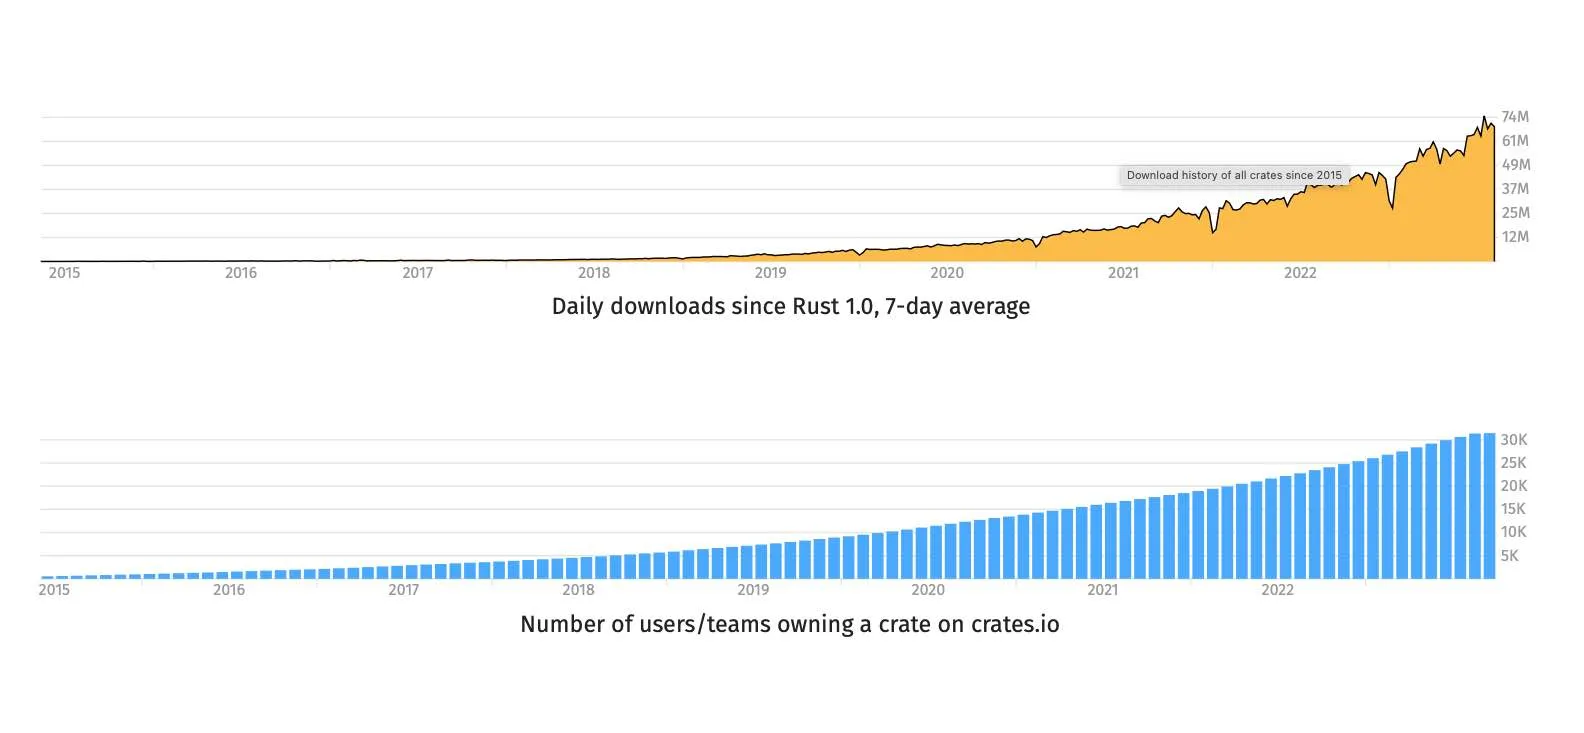
\includegraphics[width=1\linewidth]{img/lib-rs-stats-rust-downloads-users.jpg}
    \label{fig1}
\end{figure}

\indent 在并发编程方面,Rust通过线程安全的类型系统提供强有力的保障,杜绝了数据竞争问题。它的Send和Sync机制确保数据在线程间传递时符合安全规则,而所有权和借用规则使得共享数据时无需加锁或额外的同步开销,从而提升并发性能。相比于传统的锁机制,Rust还支持无数据竞争的并发模式,如基于消息传递的Actor模型和无锁数据结构,使得多线程编程更加安全高效。\\
\indent 正因为Rust在性能、内存安全和并发方面的独特优势,它成为了操作系统内核、嵌入式系统、WebAssembly、高性能计算 等领域的热门选择,并广泛应用于安全性要求极高的开发场景,如浏览器引擎(Firefox 的 Servo)、区块链(Solana)、云计算(AWS Firecracker)等。越来越多的公司和企业选择Rust语言来进行开发,如图\ref{fig1}。\\
\indent 所以我们小组计划使用Rust语言对Rt-Thread系统的部分内核进行重构,以提升系统的安全性和性能,从而更好地满足嵌入式应用的需求。\\

\subsection{当前Rust RTOS生态空缺}
当前 Rust RTOS 生态中,主要有以下几个项目:
\begin{figure}[htpb]
    \centering
    \caption{Rust RTOS生态\cite{AreWeRTOSYet}}
    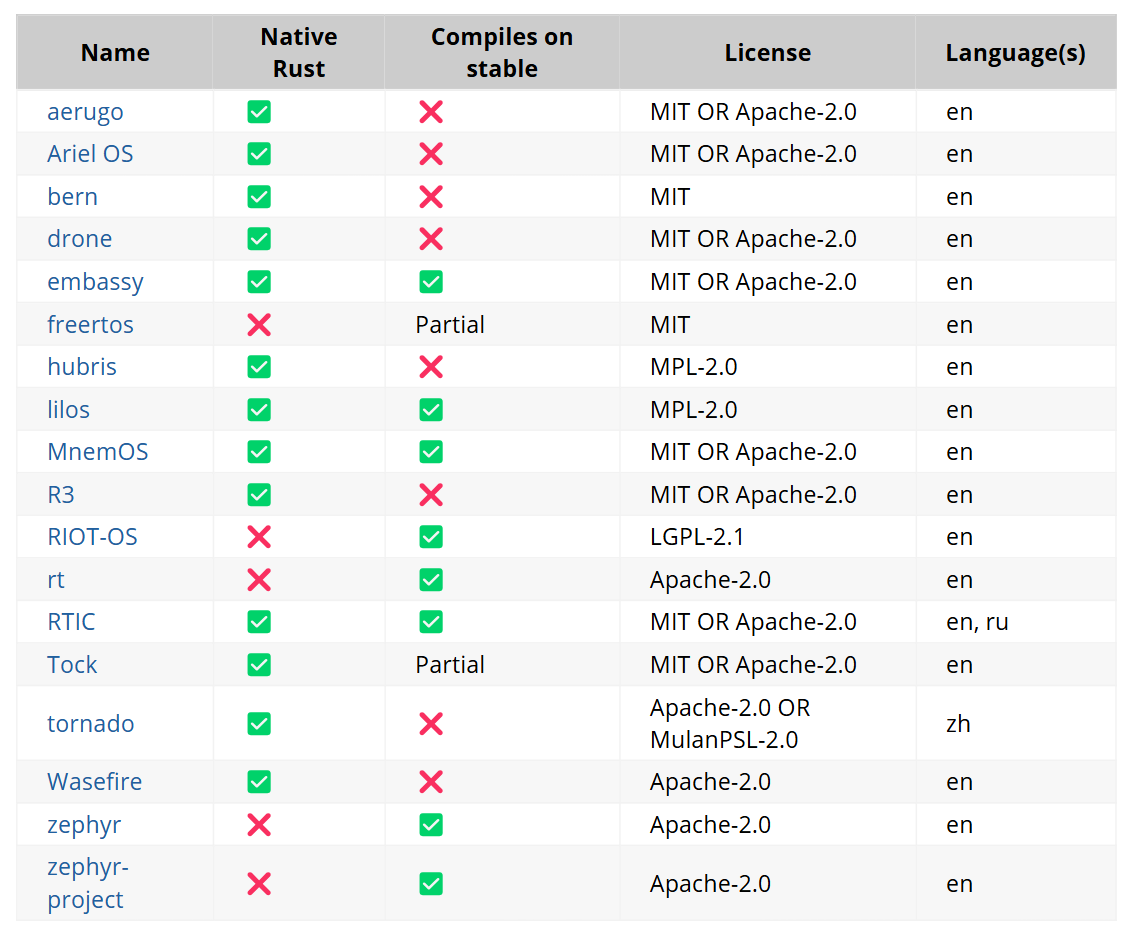
\includegraphics[width=0.5\linewidth]{img/Rust RTOS.png}
    \label{fig2}
\end{figure}

可以看出 Rust 原生实时操作系统的开发已经取得了一定的进展,但是相比于 RT-Thread 这样的成熟的嵌入式操作系统,其生态仍然不够完善。因此,将 Rust 引入 RT-Thread 这样的成熟嵌入式操作系统,将会为 Rust RTOS 生态的发展提供重要的参考和借鉴。

\section{立项依据}

\subsection{问题定义}

\textbf{核心命题}:以Rust语言重构RT-Thread Nano内核,构建兼具\textbf{安全性、实时性和开发效率}的嵌入式实时操作系统。

\subsection{重构范围}

\textbf{核心重构对象}:

\begin{itemize}
    \item 任务调度器(Scheduler):抢占式多任务调度
    \item 进程间通信(IPC):动态内存分配与碎片优化
    \item 时钟管理(Timer):信号量/消息队列同步机制
    \item 内存管理(Heap Allocator):硬件定时器与软件定时器
\end{itemize}

\subsection{技术可行性}

\subsubsection{核心模块的Rust化改造}
\textbf{Rust 调用 C 代码}
\begin{itemize}
    \item 使用 \texttt{bindgen} 自动生成 RT-Thread 内核 API 的 Rust 绑定(如 \texttt{rt\_thread\_create → unsafe extern "C"})\cite{RustBindgen}
    \item 案例参考:Linux 内核模块通过 \texttt{\#[repr(C)]} 实现结构体对齐,已验证跨语言兼容性
\end{itemize}

\textbf{C 调用 Rust 代码}
\begin{itemize}
    \item 对安全抽象层(如内存分配器)使用 \texttt{\#[no\_mangle]} 暴露接口,通过 \texttt{cbindgen} 生成 C 头文件\cite{RustCbindgen}
    \item 性能优化:在中断处理函数中采用 \texttt{\#[inline(always)]} 避免堆栈切换开销
\end{itemize}

\subsubsection{开发-调试工具链}

\textbf{编译环境}:

基于PlatformIO构建多语言工程。

{\texttt{PlatformIO Community}} 提出,PlatformIO可以自定义开发平台来支持多语言编译\cite{Kasbah_2016}。PlatformIO基于\textbf{SCons}\cite{PlatformIO_2025}进行构建,
而Scons是一个开放源码、以Python语言编码的自动化构建工具,支持集成Rust\cite{SCons}。

\textbf{仿真环境}:

\textbf{Wokwi}:Wokwi可通过配置\texttt{wokwi.toml}与\texttt{diagram.json}来模拟多种开发板与外设,方便调试与验证。\cite{Wokwi}

\textbf{调试与验证}:

PlatformIO可直接管理与真实设备的连接,并方便上板调试运行以测试。
\begin{itemize}
    \item 首阶段部署至 STM32F103C8T6 等多型号开发板(我们团队成员至少有4块不同型号的开发板),验证内核基本功能
    \item 性能对比:与原版 C 内核进行基准测试(CoreMark 得分、任务切换耗时)
\end{itemize}

\subsubsection{原项目支持}

\begin{itemize}
    \item 代码可移植性:RT-Thread Nano 内核代码量约 1.2 万行,模块化设计清晰(如 \texttt{kservice.c} 独立于硬件抽象层)\cite{RTThreadDoc}
    \item 社区支持:已有 Rust 嵌入式社区(如 \texttt{embedded-hal})提供 GPIO/UART 驱动参考
\end{itemize}

\subsection{关键点}

\begin{itemize}
    \item Rust+C编译环境的搭建
    \item RT-Thread Nano的内核结构与具体实现
    \item Rust改写
    \item 改写成果的调试验证与优化
\end{itemize}

\subsection{预期目标}

\begin{itemize}
    \item \textbf{内存安全}:通过所有权模型和借用检查,消除CWE-119(缓冲区溢出)、CWE-416(释放后使用)等漏洞。
    \item \textbf{并发安全}:Rust的\texttt{Send}/\texttt{Sync} Trait静态验证数据竞争,结合\texttt{Mutex<RefCell<T>>}智能锁,降低调度器数据竞争发生率。
    \item \textbf{性能优化}:尝试优化该系统的性能,如实时性等。
    \item \textbf{精简代码}:利用Rust的优质特性精简代码。
\end{itemize}

% Content: 重要性与前瞻性分析
% Author: 陈琳波
% Update: 2025-03-22
\section{重要性与前瞻性分析}
\subsection{C语言操作系统的安全问题}\ \\
\indent 随着物联网和嵌入式设备的快速发展,安全性和性能成为越来越重要的考虑因素。c语言以其简洁高效的特性使其成为了许多嵌入式系统和操作系统的首选。然而,C语言的低级特性也为安全问题埋下了隐患,需要我们认真对待和解决。
\subsubsection{安全问题分析}
在C语言操作系统中,常见的安全问题主要包括:
\paragraph{缓冲区溢出(Buffer Overflow):}
 当程序向缓冲区写入超出其分配空间的数据时,可能会导致数据覆盖、程序崩溃甚至远程代码执行等严重后果。\cite{17}
\paragraph{空指针解引用(Null Pointer Dereference):}
 当程序试图解引用空指针时,可能会导致程序崩溃或发生不可预测的行为,存在一定的安全风险。\cite{17}
\paragraph{内存泄漏(Memory Leaks):}
 在C语言中,动态内存的分配和释放需要由程序员手动管理,若管理不当就会导致内存泄漏问题,使得系统资源得不到释放,进而影响系统性能和稳定性。\cite{17}
\subsubsection{0day漏洞与黑客攻击}\ \\
 \indent 0day漏洞(Zero-day vulnerability): 0day漏洞是指在软件厂商尚未发现并修复的漏洞。黑客利用这些未知漏洞进行攻击,而软件开发商还没有来得及发布补丁。这类漏洞具有很高的危险性,因为黑客可以利用这些漏洞进行攻击,而用户和厂商很难发现并防范。一旦0day漏洞被公之于众,就会引起广泛关注,厂商需要尽快发布补丁来修复这些漏洞。仅在2023年,就发生了多起针对操作系统的0day漏洞攻击。\cite{15}
\paragraph{微软Windows和Office}\ \\
 \indent 2023年,微软产品曝出的最严重漏洞之一就是CVE-2023-36884(CNNVD编号:CNNVD-202307-797),这是Windows搜索工具中的远程代码执行(RCE)漏洞。该漏洞是在微软7月发布的周二补丁日中首次披露的,主要影响了Windows和Office软件。\\
\indent 与其他的微软漏洞相比,CVE-2023-36884漏洞主要有两大特点:首先,RCE漏洞在披露时没有补丁,微软仅提供了缓解措施以防止被利用,该漏洞一直到8月的周二补丁日才得到修复;其次,某东欧地区的网络犯罪组织将CVE-2023-36884用于侧重间谍的网络钓鱼活动以及出于牟利的勒索软件攻击。据微软报告,该组织的攻击目标是北美和欧洲的国防组织和政府实体。攻击者利用CVE-2023-36884绕过微软的MotW安全功能,该功能通常阻止恶意链接和附件。\cite{15}
\paragraph{苹果iOS和iPadOS}\ \\
\indent 苹果在2023年也曝出了0day漏洞,特别是9月21日披露的iOS和iPadOS中的三个漏洞尤为突出。这些漏洞包括:CVE-2023-41992(操作系统内核中的特权提升漏洞,CNNVD编号为CNNVD-202309-2064)、CVE- 2023-41991(让攻击者可以绕过签名验证的安全漏洞,CNNVD编号为CNNVD-202309-2065)以及CVE-2023-41993(苹果的WebKit浏览器引擎中导致代码任意执行的漏洞,CNNVD编号为CNNVD-202309-2063)。这些漏洞被用在一条漏洞链中,用于投放商监视供应商Cytrox的间谍软件产品Predator。埃及议会前议员Ahmed Eltantawy在2023年5月至9月期间成为了Predator间谍软件的目标。研究人员调查了其手机上的活动,发现手机感染了Predator间谍软件。
\paragraph{Linux}\ \\
\indent linux被发现了CVE-2023-0266漏洞。这是Linux 内核 ALSA 驱动中的竞争条件漏洞,可从系统用户访问,并为攻击者提供内核读写的访问权限。该漏洞是因为 ALSA 驱动程序于2017年被重构时更新了64位的函数调用而忽略了对 32 位函数调用的更新,从而将竞争条件引入了32位兼容层。Google TAG 在3月份发布报告称,针对最新版的三星Android手机的间谍活动中,该漏洞被作为包含多个 0-day 和 n-day 漏洞的利用链的一部分。\cite{15}
\subsubsection{对安全语言的渴望}\ \\
\indent 数据泄露、服务中断、财务损失......上述安全问题已经对全世界各个互联网公司造成了巨大的经济损失,因此世界迫切需要转向Rust编程语言,以提升系统的安全性和稳定性!Windows正在如日中天的rust改写windows内核,其重要性可见一斑。
\subsection{RIIR(Rewrite It In Rust)}\ \\
Rust 作为一种安全的系统语言,将语言层面的语义约束与编译器自动化推导深度结合,实现了更加严谨的编程风格和更加安全的编程方式。基于我们的分析,Rust 会成为时代的选择。
\subsubsection{编程语言回顾}\ \\
\indent 回顾过去,每一个十年,都有自己时代选择的编程语言,世界被一次又一次地改写。\\
\indent 20 世纪 60 年代:Fortran(因为 IBM!)\\
\indent 20 世纪 70 年代:BASIC(因为 Byte Magazine!) \\
\indent 20 世纪 80 年代:Pascal(因为结构化编程!) \\
\indent 20 世纪 90 年代:C++(因为面向对象!) \\
\indent 21 世纪初:Java(因为万维网!) \\
\indent 2010 年:JavaScript(因为前后端开发!) \\
\indent 2020 年:Python(因为机器学习!) \\
\indent ... \\
\indent 2030 年:Rust?
\subsubsection{Rust 对 C 的颠覆}\ \\
\indent 几年之前,微软就开始对 Rust 表现出兴趣,认为它是一种能在产品正式发布前捕捉并消除内存安全漏洞的好办法。自 2006 年以来,Windows 开发团队修复了大量由 CVE 列出的安全漏洞,其中约 70\%跟内存安全有关。\\
\indent Rust工具链一直努力防止开发者构建和发布存在安全缺陷的代码,从而降低恶意黑客攻击软件弱点的可能性。简而言之,Rust 关注内存安全和相关保护,有效减少了代码中包含的严重 bug 数量。\\
\indent 谷歌等行业巨头也已经公开对 Rust 语言示好。\\
\indent 随着业界对于内存安全编程的愈发重视,微软也在 Rust 身上显露出积极的探索热情。去年 9 月,微软发布一项非正式授权,Microsoft Azure 首席技术官 Mark Russinovich 表示新的软件项目应该使用 Rust、而非 C/C++。\\
\indent 现在,Rust 已经进入了 Windows 内核,Weston 表示微软 Windows 将继续推进这项工作,那么 Rust 很快就会得到广泛的应用。 \\
\indent 与此同时,Linux 一把手 Linus Torvalds 表示他会覆盖那些可能反对接收 Rust 代码的维护者。Linux 的二号人物 Greg Kroah-Hartman 撰写了一篇 Linux 内核邮件列表帖子,详细阐述了 Rust 的优势,并鼓励新的内核代码/驱动程序使用 Rust 而不是C 语言。\cite{Linux}
\subsection{Rust改写RT-Thread的重要性}\ \\
\indent Rust语言在操作系统开发中的应用已成为近年来技术革新的重要趋势,而将Rust引入RT-Thread这类嵌入式实时操作系统(RTOS)的改写,不仅具有现实意义,更代表了未来技术发展的方向。以下从技术、生态、行业趋势等多角度分析其重要性与前瞻性: \\
\subsubsection{技术层面的核心价值}
\paragraph{内存安全性提升}\ \\
 \indent Rust通过所有权(Ownership)和生命周期(Lifetime)机制,在编译阶段即可消除内存泄漏、野指针等常见问题。据统计,70\%的系统漏洞源于内存安全问题。例如,微软通过Rust重构Windows内核模块,显著降低了漏洞风险。对于RT-Thread这类资源受限的嵌入式系统,Rust的内存安全保障能大幅提升系统稳定性,减少因内存错误导致的崩溃或安全事件。\cite{15}
\paragraph{高性能与低开销的平衡}\ \\
 \indent Rust的零成本抽象(Zero-cost Abstraction)特性允许开发者编写高效代码,性能接近C/C++,同时避免手动管理内存的复杂性。这对于RT-Thread的实时性要求至关重要,例如线程调度、中断处理等场景需极低延迟,Rust的编译优化能力可满足此类需求。\cite{17}
\paragraph{并发编程的天然优势}\ \\
 \indent Rust通过类型系统和“无畏并发”(Fearless Concurrency)设计,简化了多线程开发。RT-Thread作为多任务实时系统,常需处理线程间同步与通信(如信号量、消息队列),Rust的并发模型可减少数据竞争风险,提升代码健壮性。\cite{17}
\subsubsection{生态与行业趋势的适配性}
\paragraph{应对AI与物联网的融合需求}\ \\
 \indent 随着端侧AI和物联网设备智能化加速,操作系统需支持更复杂的AI模型和边缘计算。Rust在高性能计算和安全性上的优势,使其成为实现AI OS的理想语言。例如,vivo的蓝河操作系统通过Rust实现了与AI大模型的深度集成,而RT-Thread若引入Rust,可更好地支持AI驱动的智能设备开发。\cite{4}
\paragraph{推动国产操作系统自主可控}\ \\
 \indent RT-Thread作为国产物联网操作系统的代表,其技术栈的自主性至关重要。Rust的现代特性与开源生态为国产系统提供了弯道超车的机会。vivo等企业通过开源Rust内核和举办创新赛事,已为国内Rust生态积累经验,RT-Thread的Rust化可借鉴此类模式,加速技术迭代。\cite{4}
\paragraph{生态工具的逐步成熟}\ \\
 \indent 当前,C/C++与Rust的互操作性工具(如代码转译)已取得突破,例如vivo创新赛中实现了项目级转译能力。这为RT-Thread逐步迁移至Rust提供了可行性。同时,Rust社区的工具链(如Cargo、Clippy)可提升开发效率,弥补嵌入式领域传统工具的不足。\cite{4}


\section{相关工作}

本项目作为计算机学院组成原理H班的大作业,完成了使用Rust改写RT-Thread国产loT操作系统内核的任务。下面将从本课程之前的Rust改写工作,国内外学术界和工业界的主流成果和本项目的创新点三个角度展开论述。

\subsection{本课程之前的Rust改写工作}

\begin{enumerate}
  \item 2019年 x-rust-freertos小组用Rust改写FreeRTOS(一个实时、嵌入式操作系统),完成了对FreeRTOS中所有的内核模块——移植(port)模块、链表(list)模块、任务调度(task)模块和队列与信号量模块的改写。
  \item 2023年 Phoenix-Flames小组用Rust改写sel4微内核,提供内存安全性和并发安全性。
  \item 2024年 mustruct小组用Rust语言重写了FreeRTOS,并在其中引入了MMU支持,以期获得更灵活、安全的内存管理能力。
  \item 2024年 mkdir小组用Rust语言重写了Linux系统的bpf-trace模块,以期能更安全地监控和分析用户空间的程序行为。
  \item 2024年 Rage\_of\_dUST小组和RushToLight小组分别用Rust语言改写了Harmony LiteOS的内存管理单元(MMU)和动态内存管理模块,提升了系统的安全性和稳定性。
\end{enumerate}

\subsection{国内外学术界和工业界对Rust改写基于C的操作系统的讨论}

\subsubsection{在Linux内核中引入Rust语言}

近年来,业界对在Linux内核中引入Rust语言表现出浓厚兴趣,主要目的是利用Rust的内存安全特性来提高内核的安全性和稳定性。然而,将Rust完全替代C来重写整个Linux内核的想法并未得到广泛支持。

目前,社区的主要工作集中在将Rust引入内核的部分模块,特别是设备驱动程序的开发。2022年,首批Rust代码被合并到Linux内核中,标志着这一尝试的开始。此后,开发者们持续推进Rust在内核中的应用,例如开发基于Rust的设备驱动程序和文件系统模块。

一些核心维护者认为Rust的内存安全特性可以减少常见的内存管理错误,提高内核的安全性和可靠性。例如,Linux内核高级开发者Greg Kroah-Hartman曾表示,添加另一种语言并非问题,关键在于项目的长期成功。他强调,使用Rust编写新代码可以减少某些类型的错误,给开发者和维护者带来益处。

然而,也有部分维护者对在内核中使用Rust持保留态度,担心多语言代码库的维护复杂性和潜在问题。例如,内核维护者Christoph Hellwig对将Rust代码引入内核表示质疑,认为这可能增加维护负担。

对此,Linux之父Linus Torvalds也曾发表看法:Linux最终不会用Rust编写,没有人会用Rust重写内核的2500万行C代码,但是他也看到了Rust的优势,鼓励采用缓慢但稳定的方法将Rust引入Linux,同时他表示将Rust接口用于驱动程序和其他非核心内核程序是有道理的。

总体而言,业界对在Linux内核中引入Rust持谨慎支持态度,认可其潜在优势,但也关注可能带来的挑战。目前的共识是,在特定模块中试验性地引入Rust,以评估其实际效果和影响。

\subsubsection{在Windows内核中引入Rust语言}

微软对在Windows内核中引入Rust持积极态度,旨在利用Rust的内存安全特性减少漏洞,提高系统安全性和性能。然而,微软并未计划全面用Rust重写整个Windows内核,而是采取逐步迁移的策略。微软Azure首席技术官Mark Russinovich曾表示,新项目应优先考虑使用Rust,而非C/C++。

具体而言,微软将Windows的文本分析、布局和渲染引擎DWriteCore部分重写为Rust版本。截至2023年,DWriteCore包含约15.2万行Rust代码和9.6万行C++代码。两名开发人员耗时半年完成了这项工作,改进后的版本已面向开发者发布。同时,微软将Win32 GDI的部分组件迁移至Rust,目前已添加了约3.6万行Rust代码。这些改进已在最新版本的Windows 11中应用,并通过了所有启动测试。

\subsubsection{其他有关Rust改写的工作}

\paragraph{Redox \href{https://www.redox-os.org/zh/?utm_source=chatgpt.com}{[redox-os.org]}}

Redox 是一个用 Rust 编程语言编写的类 Unix 微内核操作系统,旨在将 Rust 的创新(安全性、并发性和实用性)引入现代微内核和完整的应用程序生态系统。

该系统采用微内核架构,类似于 MINIX,驱动程序在用户空间运行,增强了系统的安全性和稳定性。此外,Redox 包含可选的图形用户界面 Orbital,支持 Rust 标准库,并以 MIT 许可证开源发布。

Redox 的优势主要来源于 Rust 语言的特性:极高的内存管理安全性。此外,作为一个操作系统,其通过模块化和标准化实现了可拓展性与兼容性,已经能够成为一个实际的成果而非教学用例。但是,其作为新兴操作系统还存在功能不完善、硬件支持有限、稳定性欠佳等问题。

总体而言,Redox 作为一个创新的操作系统项目,展示了 Rust 在系统开发中的潜力。尽管目前存在一些不足,但其在安全性、模块化和兼容性方面的优势,使其有继续发展的潜力。

\paragraph{TockOS \href{https://tockos.org/}{[tockos.org]}}

TockOS 是一款专为嵌入式系统设计的开源实时操作系统,采用 Rust 编程语言编写内核,旨在为无线传感器网络节点等资源受限的设备提供安全、高效的运行环境。

TockOS 的主要优势同样来自 Rust 语言的特性:类型安全和内存管理安全。同时,作为一个嵌入式操作系统,其优化了低功耗特性,满足了嵌入式设备对能耗的敏感性。同样的,作为一个新兴的操作系统,TockOS 支持的硬件十分有限,生态系统还不成熟,同时,Rust 语言高昂的学习成本也限制了其广泛使用。

\paragraph{蓝河操作系统 \href{https://blueos.vivo.com/system}{[blueos.vivo.com]}}

蓝河操作系统(BlueOS)是 vivo 于 2023 年推出的自研智慧操作系统,采用 Rust 语言编写系统框架,旨在为用户提供更智慧、更流畅、更安全的使用体验。

蓝河操作系统比起上面两个操作系统更加成熟,其借助 AI 大模型能力实现了对多模态交互的支持,包括声音、图片、文字、视频、手势等。同时,其利用 Rust 的内存安全特性,保障了系统的内存安全和并发安全。但是其仍然有应用兼容性差、生态系统成熟度低等问题。

总体而言,蓝河操作系统在智能交互和安全性方面具有显著优势,但在应用兼容性和生态系统成熟度方面仍需进一步发展。
\subsection{本项目的主要创新点}

本项目希望能将Rust引入RT-Thread,一款由中国开源社区主导开发的实时物联网操作系统。其创新点主要有以下三点:

\begin{enumerate}
  \item 相比于Linux和Windows,RT-Thread是一款嵌入式操作系统。而嵌入式操作系统相对而言由于其系统的简单性可能会更容易面临安全性挑战。而使用Rust代替C语言将从源头上解决内存管理的安全性问题。
  \item 相比于蓝河操作系统、TockOS与Redox,RT-Thread拥有更成熟的生态环境与更好的兼容性。RT-Thread已经发展了16年,其对市场上主流的硬件架构都有着很好的支持,同时,其对在线软件包管理工具的支持又让其兼具了可拓展性和兼容性。
  \item RT-Thread系统完全开源,遵循Apache License 2.0开源许可协议,并且是中国社区主持的拥有完全知识产权的产品。对RT-Thread的开发和完善有助于我国开源社区生态的发展,有助于我国操作系统自主性的实现,具有重要的战略意义。
\end{enumerate}

\section{目标与预期成果}
\begin{enumerate}
    \item \textbf{安全性重构}
    \begin{itemize}
        \item 消除 RT-Thread Nano 内核中因 C 语言缺陷导致的\textbf{7 类高危漏洞}(空指针解引用、缓冲区溢出、UAF 等)
        \item 通过 Rust 所有权模型和生命周期检查,实现\textbf{100\% 内存安全的内核核心模块}(调度器、内存管理)
    \end{itemize}
    
    \item \textbf{实时性保障}
    \begin{itemize}
        \item 在 ARM Cortex-M4 硬件平台上,确保任务调度延迟 $\leq 3\mu s$(原版 C 实现 $5\mu s$),中断响应时间 $\leq 1\mu s$
        \item 通过无锁数据结构(如 \texttt{crossbeam} 的原子队列)减少\textbf{上下文切换开销 15\%}
    \end{itemize}
    
    \item \textbf{开发效率提升}
    \begin{itemize}
        \item 利用 Rust 宏(\texttt{macro\_rules!})和泛型重构重复逻辑,减少\textbf{内核代码量 25\%}(从 12k 行 C 代码降至 9k 行 Rust 代码)
        \item 通过 \texttt{Cargo} 模块化依赖管理,实现驱动开发编译时间缩短 \textbf{30\%}
    \end{itemize}
    
    \item \textbf{生态兼容性}
    \begin{itemize}
        \item 保留 90\% 以上原有 C 语言驱动接口,通过 \texttt{bindgen/cbindgen} 工具实现\textbf{混合编程透明化}
        \item 提供 \texttt{rt-thread-sys} 和 \texttt{rt-thread-safe} 双版本 SDK,支持开发者按需选择安全等级
    \end{itemize}
\end{enumerate}

\newpage

\bibliographystyle{plain}
\bibliography{reference}

\end{document}